% Standalone, editable LaTeX/TikZ mechanism for the current ARC2-Global method.
% Visual reference: fig_arc2_mechanism_v2; computation follows src/arc2_global/model.py.
\documentclass[tikz,border=3pt]{standalone}
\usepackage[T1]{fontenc}
\usepackage{lmodern}
\usepackage{amsmath,amssymb}
\usetikzlibrary{arrows.meta,calc}
\definecolor{ink}{HTML}{253442}
\definecolor{muted}{HTML}{4F606E}
\definecolor{slate}{HTML}{2F4858}
\definecolor{frame}{HTML}{CAD3DC}
\definecolor{old}{HTML}{A9B1BB}
\definecolor{anchor}{HTML}{D9971A}
\definecolor{native}{HTML}{2E8B67}
\definecolor{proxy}{HTML}{2F6DB3}
\definecolor{query}{HTML}{8E5A9B}
\definecolor{paperblue}{HTML}{EDF3FA}
\definecolor{papergreen}{HTML}{F0F7F3}
\definecolor{papercream}{HTML}{FBF6E8}
\newcommand{\doc}[3]{%
  \fill[fill=#3] (#1,#2) rectangle ++(.068,.090);
  \draw[white,line width=.35pt] (#1+.012,#2+.058)--++(.044,0);
  \draw[white,line width=.35pt] (#1+.012,#2+.033)--++(.044,0);}
\newcommand{\vstrip}[3]{%
  \foreach \j/\a in {0/85,1/45,2/70,3/35,4/85,5/50}{
    \filldraw[fill=#3!\a,draw=#3,line width=.25pt]
      (#1+\j*.060,#2) rectangle ++(.060,.105);}}
\begin{document}
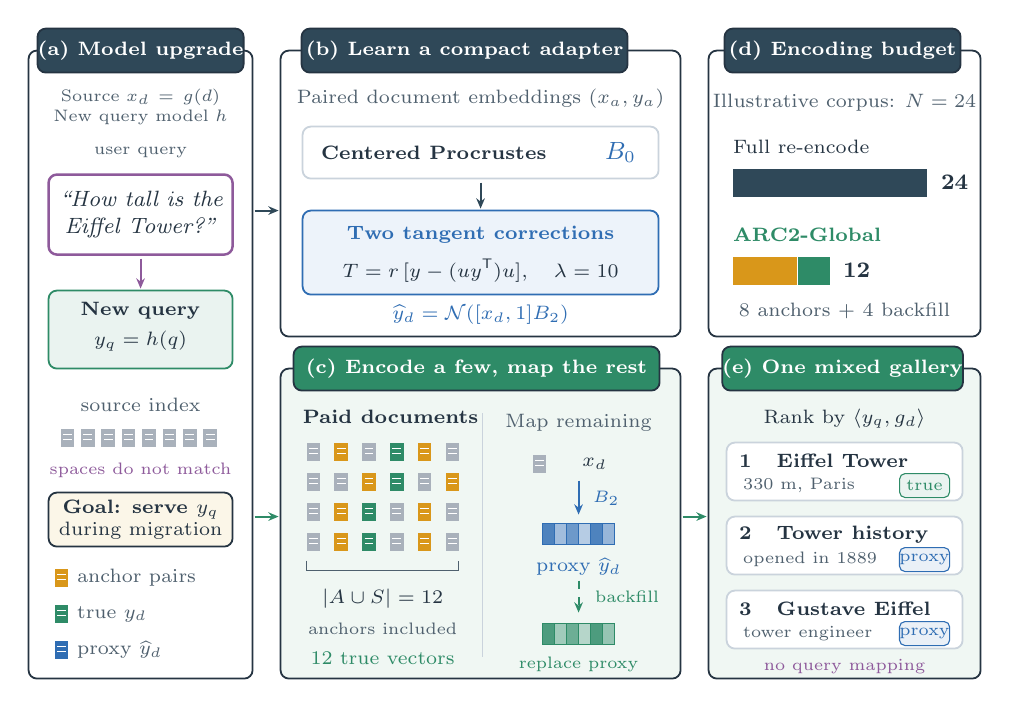
\begin{tikzpicture}[x=1in,y=1in,
  every node/.style={font=\fontsize{7}{8}\selectfont,text=ink,inner sep=0pt},
  box/.style={rounded corners=3pt,draw=ink,line width=.65pt,fill=white},
  arr/.style={-{Stealth[length=3.7pt,width=3.1pt]},line width=.75pt,draw=slate},
  small/.style={font=\fontsize{6.4}{7.3}\selectfont,text=muted},
  title/.style={font=\fontsize{7.3}{8.2}\selectfont\bfseries,text=white},
  note/.style={font=\fontsize{6.6}{7.6}\selectfont,text=muted}]

% Four editorial panels use the reference's serif typography and dark title tabs.
\draw[box] (.03,.06) rectangle (1.15,3.20);
\draw[box] (1.29,1.77) rectangle (3.29,3.20);
\draw[box,fill=papergreen] (1.29,.06) rectangle (3.29,1.61);
\draw[box] (3.43,1.77) rectangle (4.79,3.20);
\draw[box,fill=papergreen] (3.43,.06) rectangle (4.79,1.61);
\node[box,fill=slate,title,minimum height=.22in,minimum width=.96in] at (.59,3.20) {(a) Model upgrade};
\node[box,fill=slate,title,minimum height=.22in,minimum width=1.63in] at (2.21,3.20) {(b) Learn a compact adapter};
\node[box,fill=native,title,minimum height=.22in,minimum width=1.83in] at (2.27,1.61) {(c) Encode a few, map the rest};
\node[box,fill=slate,title,minimum height=.22in,minimum width=1.18in] at (4.10,3.20) {(d) Encoding budget};
\node[box,fill=native,title,minimum height=.22in,minimum width=1.18in] at (4.10,1.61) {(e) One mixed gallery};

% (a) A concrete query and the required query-space transition.
\node[small,align=center,text width=1.00in] at (.59,2.92) {Source $x_d=g(d)$\\New query model $h$};
\node[small] at (.59,2.69) {user query};
\draw[box,draw=query,line width=.9pt] (.13,2.18) rectangle (1.05,2.58);
\node[font=\fontsize{8}{10}\selectfont\itshape,align=center] at (.59,2.38) {``How tall is the\\Eiffel Tower?''};
\draw[arr,draw=query] (.59,2.16)--(.59,2.01);
\draw[box,draw=native,fill=native!10] (.13,1.61) rectangle (1.05,2.00);
\node[align=center] at (.59,1.82) {\textbf{New query}\\[3pt]$y_q=h(q)$};
\node[note] at (.59,1.43) {source index};
\foreach \i in {0,...,7}{\doc{.19+\i*.102}{1.22}{old}}
\node[small,text=query] at (.59,1.10) {spaces do not match};
\draw[box,fill=papercream] (.13,.72) rectangle (1.05,.99);
\node[align=center,font=\fontsize{6.8}{8}\selectfont] at (.59,.855) {\textbf{Goal: serve $y_q$}\\during migration};
\doc{.16}{.52}{anchor}\node[anchor=west,note] at (.27,.563) {anchor pairs};
\doc{.16}{.34}{native}\node[anchor=west,note] at (.27,.383) {true $y_d$};
\doc{.16}{.16}{proxy}\node[anchor=west,note] at (.27,.203) {proxy $\widehat y_d$};

% (b) The current global adapter: centered Procrustes, two tangent targets, collapse.
\node[note] at (2.29,2.96) {Paired document embeddings $(x_a,y_a)$};
\draw[box,draw=frame] (1.40,2.56) rectangle (3.18,2.82);
\node[anchor=west,font=\fontsize{7.2}{8}\selectfont\bfseries] at (1.49,2.69) {Centered Procrustes};
\node[text=proxy,font=\fontsize{9}{10}\selectfont] at (2.99,2.69) {$B_0$};
\draw[arr] (2.29,2.54)--(2.29,2.41);
\draw[box,draw=proxy,fill=paperblue] (1.40,1.98) rectangle (3.18,2.40);
\node[font=\fontsize{7.3}{8}\selectfont\bfseries,text=proxy] at (2.29,2.28) {Two tangent corrections};
\node[font=\fontsize{7.2}{8}\selectfont] at (2.29,2.10) {$T=r\,[y-(uy^{\mathsf T})u],\quad\lambda=10$};
\node[font=\fontsize{7.3}{8}\selectfont,text=proxy] at (2.29,1.88) {$\widehat y_d=\mathcal N([x_d,1]B_2)$};
\node[small] at (2.29,1.65) {}; % Keep explicit bounds independent of title tabs.

% (c) An illustrative 24-document budget: eight fitting anchors, four further true rows.
\node[font=\fontsize{7.1}{8}\selectfont\bfseries] at (1.84,1.37) {Paid documents};
\foreach \i in {0,...,23}{
  \pgfmathtruncatemacro{\col}{mod(\i,6)}
  \pgfmathtruncatemacro{\row}{floor(\i/6)}
  \def\dc{old}
  \ifnum\i=1 \def\dc{anchor}\fi
  \ifnum\i=4 \def\dc{anchor}\fi
  \ifnum\i=8 \def\dc{anchor}\fi
  \ifnum\i=11 \def\dc{anchor}\fi
  \ifnum\i=13 \def\dc{anchor}\fi
  \ifnum\i=16 \def\dc{anchor}\fi
  \ifnum\i=19 \def\dc{anchor}\fi
  \ifnum\i=22 \def\dc{anchor}\fi
  \ifnum\i=3 \def\dc{native}\fi
  \ifnum\i=9 \def\dc{native}\fi
  \ifnum\i=14 \def\dc{native}\fi
  \ifnum\i=20 \def\dc{native}\fi
  \doc{1.42+\col*.139}{1.15-\row*.15}{\dc}}
\draw[muted,line width=.4pt] (1.42,.65)--(1.42,.60)--(2.18,.60)--(2.18,.65);
\node[font=\fontsize{6.7}{8}\selectfont] at (1.80,.46) {$|A\cup S|=12$};
\node[small] at (1.80,.31) {anchors included};
\node[font=\fontsize{6.7}{8}\selectfont,text=native] at (1.80,.16) {12 true vectors};
\draw[frame,line width=.4pt] (2.30,.17)--(2.30,1.39);
\node[note,align=center] at (2.78,1.34) {Map remaining};
\doc{2.55}{1.09}{old}\node at (2.86,1.135) {$x_d$};
\draw[arr,draw=proxy] (2.78,1.05)--(2.78,.88);
\node[small,text=proxy,anchor=west] at (2.85,.96) {$B_2$};
\vstrip{2.60}{.73}{proxy}
\node[note,text=proxy] at (2.78,.62) {proxy $\widehat y_d$};
\draw[arr,draw=native,dashed] (2.78,.55)--(2.78,.39);
\node[small,text=native,anchor=west] at (2.86,.47) {backfill};
\vstrip{2.60}{.23}{native}
\node[small,text=native] at (2.78,.13) {replace proxy};

% (d) Counts in the toy, not timings or measured deployment savings.
\node[note] at (4.11,2.94) {Illustrative corpus: $N=24$};
\node[anchor=west] at (3.55,2.72) {Full re-encode};
\fill[slate] (3.55,2.47) rectangle (4.52,2.61);
\node[anchor=west,font=\fontsize{7.7}{8}\selectfont\bfseries] at (4.59,2.54) {24};
\node[anchor=west,text=native,font=\fontsize{7.2}{8}\selectfont\bfseries] at (3.55,2.28) {ARC2-Global};
\fill[fill=anchor] (3.55,2.03) rectangle (3.8733,2.17);
\fill[native] (3.8733,2.03) rectangle (4.0350,2.17);
\draw[white,line width=.5pt] (3.8733,2.03)--(3.8733,2.17);
\node[anchor=west,font=\fontsize{7.7}{8}\selectfont\bfseries] at (4.10,2.10) {12};
\node[note] at (4.11,1.90) {8 anchors $+$ 4 backfill};

% (e) Schematic hits demonstrate that mapped documents remain searchable.
\node[font=\fontsize{6.8}{8}\selectfont] at (4.11,1.36) {Rank by $\langle y_q,g_d\rangle$};
\foreach \y/\rk/\name/\snippet/\lab/\cc in {
  .95/1/{Eiffel Tower}/{330 m, Paris}/{true}/native,
  .58/2/{Tower history}/{opened in 1889}/{proxy}/proxy,
  .21/3/{Gustave Eiffel}/{tower engineer}/{proxy}/proxy}{
  \draw[box,draw=frame] (3.52,\y) rectangle (4.70,\y+.29);
  \node[anchor=west,font=\fontsize{7.1}{8}\selectfont\bfseries] at (3.58,\y+.20) {\rk\quad\name};
  \node[anchor=west,small] at (3.60,\y+.075) {\snippet};
  \node[rounded corners=2pt,draw=\cc,fill=\cc!10,text=\cc,
    minimum width=.25in,minimum height=.12in,
    font=\fontsize{5.9}{6.5}\selectfont] at (4.51,\y+.075) {\lab};}
\node[small,text=query] at (4.11,.12) {no query mapping};

% Reading flow between the editorial panels.
\draw[arr] (1.16,2.40)--(1.28,2.40);
\draw[arr,draw=native] (1.16,.87)--(1.28,.87);
\draw[arr,draw=native] (3.30,.87)--(3.42,.87);
\end{tikzpicture}
\end{document}
